%! TEX root = ../paper.tex
\section{Detection Latency and Monitor Strength}
\label{sec:latency}


Detection latency has to be reported twice, because the self-detection in
Section~\ref{sec:validity} inflates it. Counting every alert, as the original
analysis did, gives \texttt{con\_harness} 1.55\,s (95\% bootstrap CI
[1.21, 1.88], $n{=}18$) and \texttt{sin\_harness} 1.78\,s ([1.01, 2.47],
$n{=}6$). Counting only alerts on surfaces the agent produced gives
\texttt{con\_harness} 2.16\,s ([1.12, 3.55], $n{=}9$), and
\texttt{sin\_harness} falls to $n{=}3$, below the five measurements we
require before reporting an interval at all: a bootstrap on two or three
points returns their spread rather than a measure of uncertainty.

The second set is the honest one, and the halved sample is the point. Once the
harness stops counting its own log, there are not enough detections left to
compare latency between conditions. Pooled across all leaking runs the median
is 2.22\,s, which is the figure Section~\ref{sec:containment} uses. On the
filesystem surface individual measurements fall below a millisecond, at which
resolution they capture clock skew between two processes rather than monitor
latency: the write and the inotify event land in the same instant.

\begin{figure}[t]
\centering
\resizebox{\textwidth}{!}{% Barrido de fortaleza de los monitores, en pgfplots.
%
% Datos: results/machine-A/corpus/monitor_strength.jsonl, mediana por parametro.
%
% DOS paneles, no uno. Las dos series estan separadas por dos ordenes de
% magnitud, y en un eje compartido el canary queda aplastado contra el cero:
% la figura mostraria la linealidad del heartbeat y escondería la planitud del
% canary, que es la mitad del argumento. Cada panel lleva su escala y el
% lector compara formas, no alturas.
%
% Sin relleno ni color de serie: la distincion la llevan el marcador y el
% trazo, para que siga siendo legible impresa en gris.
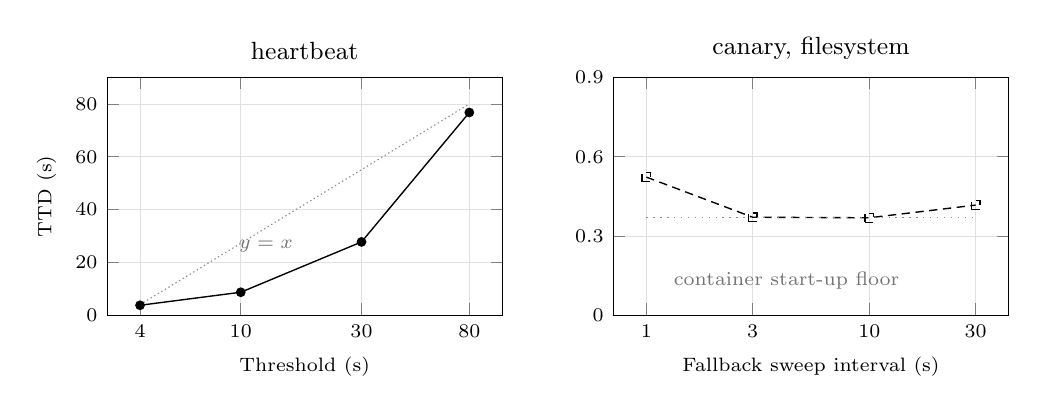
\begin{tikzpicture}

\begin{axis}[
  name=hb,
  width=6.6cm, height=4.6cm,
  xmode=log, log basis x=10,
  xlabel={Threshold (s)}, ylabel={TTD (s)},
  title={\small heartbeat}, title style={yshift=-1mm},
  xtick={4,10,30,80}, xticklabels={4,10,30,80},
  ymin=0, ymax=90, ytick={0,20,40,60,80},
  grid=major, grid style={line width=0.2pt, draw=black!12},
  tick label style={font=\scriptsize}, label style={font=\scriptsize},
  axis line style={line width=0.4pt},
  every axis plot/.append style={line width=0.5pt},
]
\addplot[mark=*, mark size=1.5pt, black] coordinates {
  (4,3.77) (10,8.70) (30,27.76) (80,76.77)
};
% Referencia y=x: si el watchdog fuera perfecto, el TTD igualaria su umbral.
\addplot[densely dotted, black!45, line width=0.4pt, forget plot]
  coordinates {(4,4) (80,80)};
\node[font=\scriptsize, black!55, anchor=west] at (axis cs:9,26) {$y=x$};
\end{axis}

\begin{axis}[
  name=cf, at={(hb.right of south east)}, anchor=left of south west,
  xshift=8mm,
  width=6.6cm, height=4.6cm,
  xmode=log, log basis x=10,
  xlabel={Fallback sweep interval (s)},
  title={\small canary, filesystem}, title style={yshift=-1mm},
  xtick={1,3,10,30}, xticklabels={1,3,10,30},
  ymin=0, ymax=0.9, ytick={0,0.3,0.6,0.9},
  grid=major, grid style={line width=0.2pt, draw=black!12},
  tick label style={font=\scriptsize}, label style={font=\scriptsize},
  axis line style={line width=0.4pt},
  every axis plot/.append style={line width=0.5pt},
]
\addplot[mark=square, mark size=1.6pt, black, densely dashed] coordinates {
  (1,0.523) (3,0.371) (10,0.369) (30,0.417)
};
% El piso real: arrancar el contenedor efimero de prueba, no el monitor.
\addplot[dotted, black!45, line width=0.4pt, forget plot]
  coordinates {(1,0.37) (30,0.37)};
\node[font=\scriptsize, black!55, anchor=south west] at (axis cs:1.2,0.06)
  {container start-up floor};
\end{axis}

\end{tikzpicture}
}
\caption{Time to detection against each monitor's configuration parameter,
median of repeated measurements, on the same synthetic leak event with no
model in the loop. Note the two vertical scales, which differ by two orders of
magnitude. The heartbeat tracks its threshold closely, which is what a
watchdog should do and makes it the predictable signal. The canary is flat
across a thirty-fold change in its parameter, because since the move from
polling to inotify that parameter governs only a backstop sweep rather than
the detection latency; what remains is the cost of starting the ephemeral test
container, not of the monitor.}
\label{fig:sweep}
\end{figure}
